\chapter{Performance Analysis}

In this section, we present the results of our proposed acceleration techniques and describe the fitness function used across all experiments. The goal of our fitness function is to balance predictive performance with hardware efficiency, ensuring that the selected models are not only accurate but also suitable for deployment on resource-constrained devices.

The fitness function is defined as:

\begin{equation}
\text{Fitness} =
\begin{cases}
\begin{aligned}
0.7 \cdot \text{Accuracy}_{\text{TFLite}} 
+ 0.2 \cdot \left(1 - \dfrac{\text{RAM}}{\text{MaxRAM}}\right) \\
+ 0.1 \cdot \left(1 - \dfrac{\text{Flash}}{\text{MaxFlash}}\right),
\end{aligned}
& \text{if } \text{RAM} \leq \text{MaxRAM} \land \text{Flash} \leq \text{MaxFlash} \\
-1000, & \text{otherwise}
\end{cases}
\label{eq:fitness_function}
\end{equation}



This formulation was chosen to explicitly incorporate hardware constraints into the optimization objective. Including this fitness function, we effectively guide the Genetic Algorithm (GA) to prioritize models that are not only accurate but also memory-efficient.

Notably, although the highest accuracy achieved during training (at 70 epochs) was approximately 65\%, the fitness function allows models with lower accuracy (e.g., around 40\%) to outperform others if they demonstrate significantly lower memory usage. However, by assigning a higher weight (0.7) to the accuracy term in the fitness function, we ensure that performance remains the primary objective. This is especially important considering that accuracy typically ranges from 0.3 to 0.65, while the normalized RAM and Flash components can span from 0 to 0.85. Without the weighted terms, the smallest models would consistently dominate the selection process—regardless of their predictive performance. The chosen weighting strategy ensures that the evolutionary search favors architectures that are not only compact and efficient but also sufficiently accurate for deployment.

It's important to note that microcontrollers are typically designed for specific tasks within embedded systems, combining processing, memory, and input/output peripherals on a single chip. This design makes them cost-effective and power-efficient for dedicated applications . In such scenarios, as long as the model fits within the available memory constraints of the microcontroller, such as the 256KB SRAM of the Arduino Nano 33 BLE Sense , the exact memory consumption becomes less critical. Therefore, the fitness function's weighting ensures a balance between model accuracy and resource efficiency, aligning with the practical considerations of deploying models on resource-constrained devices \cite{arduino_nano33ble}.



\section{Memory Estimation Experiment}

To assess the effectiveness of the proposed memory-aware optimization, a dedicated experiment was conducted in which the memory filtering mechanism was deliberately disabled. In this configuration, models exceeding the allowable RAM or flash memory constraints were not filtered out prior to training. Instead, any model violating the hardware limits was penalized post-training by assigning it a fixed fitness value of –1000. The purpose of this experiment was to investigate whether the genetic algorithm (GA) could inherently learn to avoid infeasible models, despite the lack of preemptive filtering.

Following a 4-hour NAS run, it became evident that only a limited number of models were successfully trained. This was primarily due to the fact that models with larger RAM and flash memory requirements consumed significantly more computational time—even for short training durations. In some cases, a single large model required up to four times the training time of a smaller, resource-efficient one (see Table~\ref{tab:taku_models}). This disparity in training time illustrates the inefficiency introduced by allowing oversized models to enter the search process.

Moreover, after evaluating all trained models, only a small fraction were found to be deployable on the Arduino Nano. While the RankNet-based predictor demonstrated some ability to identify promising architectures before training, its utility was limited in scenarios where the vast majority of candidates were infeasible. Specifically, when many models received the same penalty score (e.g., –1000), the RankNet network struggled to make meaningful comparisons during pairwise ranking. This led to stagnation in the learning process, as the predictor could not effectively differentiate between models based solely on invalid fitness values.

As illustrated in Figure~\ref{fig:memoryEstimationTest}, approximately \textbf{75\%} of the trained models were ultimately undeployable due to violating memory constraints. This result highlights the substantial inefficiencies introduced when memory-aware filtering is not applied. Beyond wasting training time on models that will later be discarded, the overall search process is slowed due to longer training cycles and increased difficulty in selecting promising candidates. Incorporating early memory estimation not only improves the efficiency of NAS by avoiding wasted computation, but also ensures that the evolutionary search is guided more effectively toward viable, deployable solutions.

\clearpage

\begin{table}[ht]
\noindent % removes indentation
\hspace*{-\oddsidemargin} % shift left based on page margin
\makebox[\linewidth][l]{%
\resizebox{1.20\textwidth}{!}{%
\begin{tabular}{|l|c|c|c|c|c|c|c|c|c|c|c|c|c|c|c|}
\hline
\textbf{Model} & \textbf{Train Acc} & \textbf{Test Acc} & \textbf{SWA Acc} & \textbf{TFLite Acc} & \textbf{Opt.} & \textbf{Precision} & \textbf{Recall} & \textbf{F1} & \textbf{RAM (KB)} & \textbf{Flash (KB)} & \textbf{TFLite (KB)} & \textbf{FLOPs} & \textbf{Fitness} & \textbf{Time (min)} & \textbf{Epochs} \\
\hline
TakuNet\_Init\_0 & 0.8922 & 0.5717 & 0.5717 & 0.5730 & adamw & 0.5712 & 0.5717 & 0.5690 & 546.91 & 15020.00 & 13731.02 & 31824133 & -1000.00 & 14.48 & 10 \\
TakuNet\_Mutant\_13 & 0.4719 & 0.4396 & 0.4396 & 0.4367 & adamw & 0.4342 & 0.4396 & 0.4304 & 52.18 & 316.71 & 321.56 & 750018 & 0.5130 & 4.92 & 10 \\
\hline
\end{tabular}
}}
\caption{Performance summary of two TakuNet models.}
\label{tab:taku_models}
\end{table}

\bigskip

\begin{figure}[ht]
    \centering
    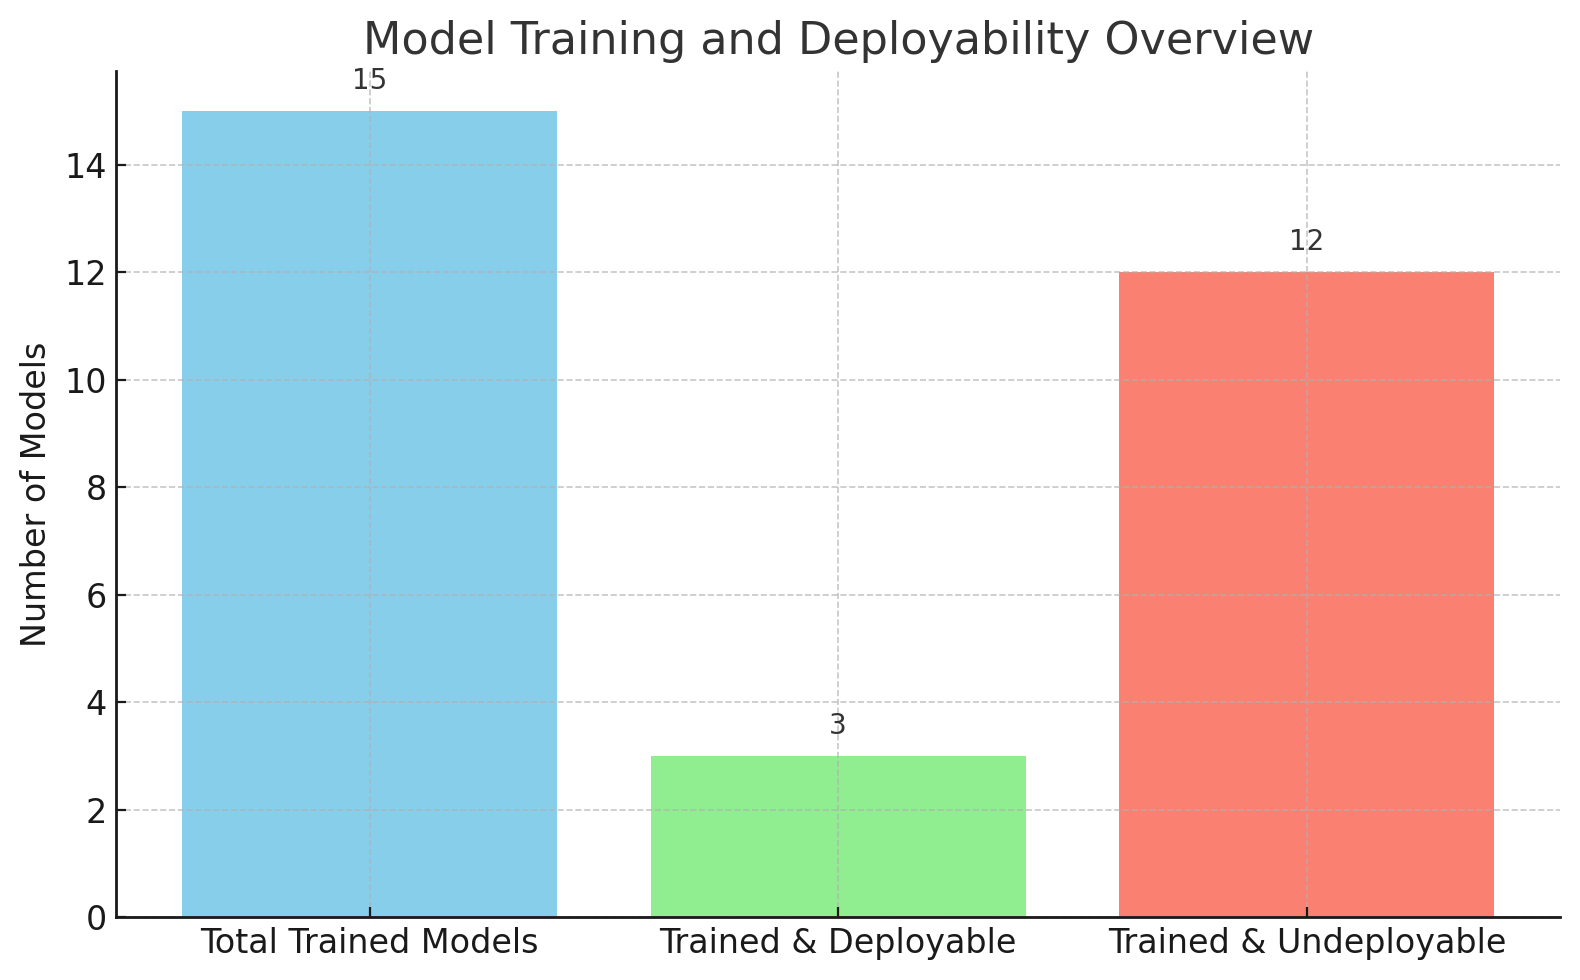
\includegraphics[width=0.85\linewidth]{Pictures/MemoryEstimationTest.png}
    \caption{MemoryEstimationTest}
    \label{fig:memoryEstimationTest}
\end{figure}





\section{Performance Stop Experiment}



\section{Early Stoppage Experiment}
In this experiment, we as on the above we aimed to stop the training of specific models, with the goal to reduce the training time, if we know that the performance will not be very good. As explained the first couple of epochs are the most significant ones. If the model does not reach a specific percentile of the highest possible accuracy we can be certain that it does not worth to spend more time training this model.


\section{RankNet Experiment}

In this experiment, we analyzed the results from a large-scale NAS run that lasted approximately 9 hours. Since our comparisons are based on tournament selection, it is nearly impossible to replicate the exact pairwise matchup encountered during the original run. To ensure transparency, we retained both the fitness values and the parameter configurations of every model evaluated.

We then performed random pairwise comparisons between models to assess how accurately the RankNet model could predict which architecture would perform better.

It is also important to note that in our NAS algorithm, some of RankNet's potential misjudgments are mitigated. Specifically, we only fully rely on its predictions when both competing models have not yet been trained, making the actual implementation even more accurate than what we see in the experiment.





\TODO{What this section must have

1) Make a RUN1 for a day using 50epochs, then make a code to run all the models for 10,20,30 epochs to show the idea of the learning Rate.
Compare the results, and prove that you can correctly predict models

2) Try to measure the current

3) Try to see if any comparisons would be saved (Though as we dont know in advance with duels are going to happen)

!!! You also have to modify the fitness function, to give very pure results for each model outside of the boundaries

4) Make a second big run without any filters (or maybe just add the Memory Estimation),get the results, see how many Models would be stopped.

1) You have to modify the Early Stoppage
2) Can I somehow show the RankNet Result?

}